\documentclass[conference]{IEEEtran}
\IEEEoverridecommandlockouts
% The preceding line is only needed to identify funding in the first footnote. If that is unneeded, please comment it out.
\usepackage{cite}
\usepackage{amsmath,amssymb,amsfonts}
\usepackage{algorithmic}
\usepackage{graphicx}
\usepackage{textcomp}
\usepackage{xcolor}
\def\BibTeX{{\rm B\kern-.05em{\sc i\kern-.025em b}\kern-.08em
    T\kern-.1667em\lower.7ex\hbox{E}\kern-.125emX}}

\usepackage{cite}
\usepackage{amsmath,amssymb,amsfonts}
\usepackage{algorithmic}
\usepackage{graphicx}
\usepackage{textcomp}
\usepackage{xcolor}

\begin{document}

\title{Depo Yeri Seçimi Probleminde K-Means ve Greedy Yaklaşım Tabanlı Hibrit Bir Optimizasyon Algoritması}

\author{
    \IEEEauthorblockN{Sena Nur Bahçevan}
    \IEEEauthorblockA{\textit{Yazılım Mühendisliği Bölümü} \\
    \textit{Manisa Celal Bayar Üniversitesi}\\
    Manisa, Türkiye \\
    sena.bahcevan@example.com}
    \and
    \IEEEauthorblockN{Gülsu Beşe}
    \IEEEauthorblockA{\textit{Yazılım Mühendisliği Bölümü} \\
    \textit{Manisa Celal Bayar Üniversitesi}\\
    Manisa, Türkiye \\
    gulsu.bese@example.com}
}

\maketitle

\begin{abstract}

Depo Yeri Seçimi Problemi (Warehouse Location Problem - WLP), müşteri taleplerine en düşük maliyetle hizmet verecek depo konumlarının belirlenmesini amaçlayan önemli bir lojistik problemidir. Bu çalışmada, tek bir algoritmanın yetersiz kaldığı durumlarda daha etkili çözümler üretebilmek amacıyla K-Means kümeleme algoritması ile Greedy (Açgözlü) yaklaşımı birleştiren hibrit bir yöntem önerilmiştir. İlk aşamada müşteri lokasyonları K-Means algoritması kullanılarak kümelere ayrılmış, ikinci aşamada ise her küme için merkeze en yakın gerçek müşteri noktası greedy yaklaşımıyla depo konumu olarak belirlenmiştir. Ayrıca modele depo kurulum maliyetleri de dahil edilerek daha gerçekçi bir lojistik yapı oluşturulmuştur. Önerilen hibrit yöntemin performansı farklı depo sayıları ($K$) altında Random Search yöntemi ile karşılaştırılmıştır. Elde edilen sonuçlar, hibrit yaklaşımın toplam maliyeti azaltmada daha başarılı ve kararlı sonuçlar ürettiğini göstermektedir.

\end{abstract}

\begin{IEEEkeywords}
Depo Yeri Seçimi Problemi, K-Means Kümeleme, Greedy Algoritma, Lojistik Optimizasyonu.
\end{IEEEkeywords}

\section{Giriş}

Günümüzde lojistik ve tedarik zinciri yönetimi, organizasyonların rekabet avantajı elde etmesinde kritik bir rol oynamaktadır. Özellikle depo ve dağıtım merkezleri, ürünlerin üreticiden müşteriye ulaştırılması sürecinde stratejik bir bağlantı noktası olarak görev yapmaktadır. Bu nedenle depo yeri seçimi problemi, yalnızca lojistik maliyetleri değil aynı zamanda tedarik zincirinin genel performansını doğrudan etkileyen önemli bir optimizasyon problemi olarak değerlendirilmektedir \cite{owen1998strategic,sagnak2020depo}.
 
Depo yeri seçimi problemi (Warehouse Location Problem - WLP), belirli bir bölgede coğrafi olarak dağılmış müşteri taleplerine minimum toplam maliyet ile hizmet verecek depo konumlarının belirlenmesini amaçlamaktadır \cite{you2019optimal}. Organizasyonların toplam giderlerinin önemli bir kısmı taşıma ve dağıtım maliyetlerinden oluştuğu için, tesis yeri seçimi stratejik karar süreçlerinde büyük önem taşımaktadır. Bu nedenle problem, literatürde p-medyan, kümeleme, matematiksel programlama ve sezgisel yöntemler gibi farklı yaklaşımlarla ele alınmıştır \cite{karagul2014pmedyan}.
 
Ancak depo yeri seçimi problemi yüksek boyutlu ve karmaşık yapısı nedeniyle çözülmesi zor optimizasyon problemleri arasında yer almaktadır. Literatürde yaygın olarak kullanılan ağırlıklı K-Means algoritması hızlı sonuç üretmesine rağmen başlangıç noktalarına duyarlı olması ve çoğu zaman yerel optimum çözümlere takılması önemli dezavantajlar oluşturmaktadır. Literatürdeki çalışmalar, K-Means tabanlı çözümlerin başlangıç parametrelerine bağlı olarak optimum sonuçlardan kayda değer oranlarda sapabildiğini göstermektedir \cite{you2019optimal}. Bu durum, daha etkili ve esnek çözüm yaklaşımlarına olan ihtiyacı artırmaktadır.
 
Bu çalışmanın temel amacı, sürekli bir düzlemde dağılmış müşteri kitlelerine en düşük maliyetle hizmet verecek optimum depo konumlarını belirlemektir. Bu kapsamda K-Means kümeleme algoritması ile greedy (açgözlü) yaklaşımı birleştiren hibrit bir yöntem geliştirilmiştir. Geliştirilen yöntem iki aşamalı bir karar mekanizması yürütmektedir. İlk aşamada, gözetimsiz öğrenme yöntemlerinden biri olan K-Means algoritması kullanılarak müşteriler geometrik kümelere ayrılmaktadır. İkinci aşamada ise her kümenin teorik merkez noktası, lojistik uygulanabilirliği artırmak amacıyla ilgili kümeye en yakın gerçek müşteri lokasyonuna greedy yaklaşımıyla eşlenmektedir. Böylece teorik merkezler yerine gerçek hayatta uygulanabilir depo noktaları elde edilmektedir.
 
Ayrıca çalışmada geliştirilen hibrit algoritmanın performansı Random Search yöntemi ile karşılaştırılmıştır. Yapılan deneysel analizler sonucunda hibrit yaklaşımın toplam taşıma maliyetini önemli ölçüde azalttığı ve daha dengeli çözümler ürettiği gözlemlenmiştir. Elde edilen sonuçlar, hibrit yöntemlerin depo yeri seçimi gibi karmaşık optimizasyon problemlerinde etkili bir alternatif oluşturabileceğini göstermektedir.

\section{Literatür Taraması}

Depo Yeri Seçimi Problemi (Warehouse Location Problem - WLP), tesis yeri seçimi problemlerinin en önemli alt başlıklarından biri olup lojistik, tedarik zinciri yönetimi ve yöneylem araştırması alanlarında uzun yıllardır yoğun biçimde çalışılmaktadır. Literatürde tesis yeri seçimi problemleri çoğunlukla p-medyan modelleri ve varyasyonları üzerinden ele alınmıştır. Literatürde, p-medyan modellerinin temel amacının belirli müşteri taleplerini minimum toplam maliyet ile karşılayacak tesis konumlarının belirlenmesi olduğu ifade edilmiştir \cite{karagul2014pmedyan}. Ancak problem yapısının kombinatoryal olması ve çözüm uzayının hızlı büyümesi nedeniyle WLP, NP-Hard sınıfında değerlendirilen zor optimizasyon problemleri arasında yer almaktadır.
 
Depo yeri seçimi problemlerinin çözümünde literatürde matematiksel programlama yöntemleri, sezgisel algoritmalar, meta-sezgisel yöntemler ve çok kriterli karar verme teknikleri yaygın olarak kullanılmaktadır \cite{sagnak2020depo}. Özellikle büyük ölçekli problemlerde kesin çözüm yöntemlerinin yüksek hesaplama maliyetine sahip olması nedeniyle araştırmacılar daha hızlı sonuç üretebilen sezgisel yöntemlere yönelmiştir.
 
Literatürdeki çalışmalar incelendiğinde, eşzamanlı depolamada uyumlu ürünlerin saklanabilmesi için gerekli minimum depo sayısını belirlemeye yönelik sezgisel yaklaşımlar geliştirildiği görülmektedir \cite{kalfakakou2003minimum}. Depo yeri problemi için basit ve etkili bir tabu arama algoritması önerilirken \cite{michel2004simple}, depo yeri ve perakendeci tahsisi problemini 0-1 tam sayılı programlama modeli olarak ele alan ve büyük ölçekli problemlerde kullanılmak üzere iki aşamalı sezgisel bir çözüm yaklaşımı sunan çalışmalar da mevcuttur \cite{gill2007optimal}.
 
Meta-sezgisel yöntemlerin kullanıldığı çalışmalar da literatürde önemli bir yer tutmaktadır. Otomobil yedek parça deposu yer seçimi probleminde mevcut depolama alanını en üst düzeye çıkarmak ve optimum tahsis işlemleri için Parçacık Sürü Optimizasyonu (PSO) yöntemi kullanılmıştır \cite{yaobao2013improved}. Açılacak depoların yerini, kapasite seviyesini, dağıtım yollarını ve stok miktarlarını belirlemek amacıyla genetik algoritma tabanlı yaklaşımlar geliştirilmiştir \cite{askin2014multi}. Afet yardım lojistiğinde depo yeri-yönlendirme problemini çözmek amacıyla matematiksel sezgisel (math-heuristic) bir yöntem önerilirken \cite{rath2014math}, aktif setli güven bölgesi algoritması kullanarak toplam dağıtım maliyetini minimize edecek servis merkezi sayılarını ve büyüklüklerini belirlemeye çalışan araştırmalar da bulunmaktadır \cite{aboelnaga2017active}.
 
Son yıllarda veri odaklı yöntemlerin gelişmesiyle birlikte makine öğrenmesi tabanlı yaklaşımlar da depo yeri seçim problemlerinde kullanılmaya başlanmıştır. Özellikle K-Means kümeleme algoritması, müşteri lokasyonlarını hızlı ve düşük maliyetli şekilde gruplandırabilmesi nedeniyle dikkat çekmektedir. Bununla birlikte K-Means algoritmasının oluşturduğu küme merkezlerinin teorik noktalar olması ve gerçek hayatta fiziksel karşılıklarının bulunmaması önemli bir dezavantaj olarak değerlendirilmektedir. Literatürdeki çalışmalar, ağırlıklı K-Means yönteminin başlangıç noktalarına duyarlı olduğunu ve bazı durumlarda optimum çözümden önemli ölçüde sapabildiğini doğrulamaktadır \cite{you2019optimal}.
 
Literatürde depo yeri seçimi problemlerinde kümeleme tabanlı yöntemler, sezgisel algoritmalar ve meta-sezgisel yaklaşımların yaygın olarak kullanıldığı görülmektedir. Özellikle K-Means algoritması hızlı ve düşük maliyetli çözümler üretebilmesi açısından dikkat çekmektedir. Ancak bazı çalışmalarda küme merkezlerinin teorik noktalarda kalması, elde edilen sonuçların fiziksel uygulanabilirliği açısından sınırlılıklar oluşturabilmektedir. Bu çalışmada ise K-Means algoritmasının hızlı kümeleme yeteneği, greedy (açgözlü) yaklaşım ile desteklenerek daha uygulanabilir depo konumları elde edilmesi amaçlanmıştır. Ayrıca önerilen hibrit yaklaşımın performansı Random Search yöntemi ile karşılaştırılarak toplam maliyet üzerindeki etkisi analiz edilmiştir.

\section{Yöntem}

Bu çalışmada önerilen hibrit çözüm modeli, sürekli bir düzlemde dağılmış müşteri lokasyonları için optimum depo konumlarını belirlemek amacıyla iki aşamalı bir yapı kullanmaktadır. Modelin ilk aşamasında müşteri noktaları K-Means kümeleme algoritması ile mantıksal hizmet bölgelerine ayrılmakta, ikinci aşamada ise greedy (açgözlü) yaklaşım kullanılarak fiziksel olarak uygulanabilir depo konumları belirlenmektedir. Geliştirilen hibrit yapı sayesinde hem hesaplama maliyetinin azaltılması hem de gerçek dünya koşullarına uygun depo konumlarının elde edilmesi amaçlanmaktadır.

\subsection{K-Means Tabanlı Bölümleme}

K-Means algoritması, basit uygulanabilirliği ve hızlı çalışması nedeniyle en yaygın kullanılan kümeleme algoritmalarından biridir \cite{kmeans}. Algoritmanın temel amacı, $n$ adet veri noktasını önceden belirlenen $K$ adet kümeye ayırarak küme içi benzerliği maksimize etmektir.
 
Algoritmanın ilk adımında, $N = 300$ adet müşteriden oluşan veri kümesi, gözetimsiz öğrenme yöntemlerinden K-Means algoritması ile $K$ adet mantıksal hizmet bölgesine ayrılmaktadır. K-Means algoritması, her bir müşterinin seçilen küme merkezine olan Öklid uzaklıklarının kareleri toplamını minimize etmeyi amaçlar. Amaç fonksiyonu Denklem (1)'de gösterilmektedir:
 
\begin{equation}
J = \sum_{i=1}^{K} \sum_{x \in S_i} \|x - \mu_i\|^2
\end{equation}
 
Burada $K$ toplam küme sayısını, $S_i$ ilgili kümeye ait müşteri kümesini, $x$ müşteri koordinat vektörünü ve $\mu_i$ ise ilgili kümenin merkez noktasını temsil etmektedir.
 
Algoritma iteratif olarak çalışmaktadır. İlk aşamada rastgele başlangıç merkezleri seçilmekte, daha sonra her müşteri en yakın merkeze atanmakta ve yeni merkez noktaları hesaplanmaktadır. Bu süreç, merkez konumları değişmeyene kadar tekrar edilmektedir. Konum belirleme ve atama işlemleri arasında dönüşümlü olarak devam eden bu süreç iyileşme kalmayana kadar sürdürülmektedir \cite{salhi2003genetic}.

\subsection{Greedy (Açgözlü) Depo Konumlandırma}

K-Means algoritması sonucunda elde edilen küme merkezleri sürekli uzayda teorik noktalar olarak oluşmaktadır. Ancak bu merkez noktalarının fiziksel olarak kullanılabilir olmaması lojistik açıdan önemli bir problem oluşturmaktadır.
 
Bu problemi çözmek amacıyla çalışmada greedy (açgözlü) tabanlı bir depo seçim mekanizması geliştirilmiştir. Her küme için, ilgili kümedeki gerçek müşteri lokasyonlarının teorik merkez noktasına olan Öklid uzaklıkları hesaplanmaktadır. Ardından merkeze en yakın gerçek müşteri noktası nihai depo konumu olarak seçilmektedir. Bu işlem Denklem (2)'de ifade edilmektedir:
 
\begin{equation}
W_i = \arg\min_{p \in S_i} \|p - \mu_i\|
\end{equation}
 
Burada $W_i$ ilgili küme için seçilen depo konumunu, $p$ müşteri lokasyonlarını ve $\mu_i$ küme merkezini göstermektedir. Önerilen greedy yaklaşım sayesinde arama uzayı yalnızca mevcut müşteri lokasyonları ile sınırlandırılmış ve fiziksel olarak uygulanabilir depo noktaları elde edilmiştir.

% --------------------------------------------------
% GÖRSELLERİN EKLENMESİ
% --------------------------------------------------
\begin{figure}[htbp]
\centerline{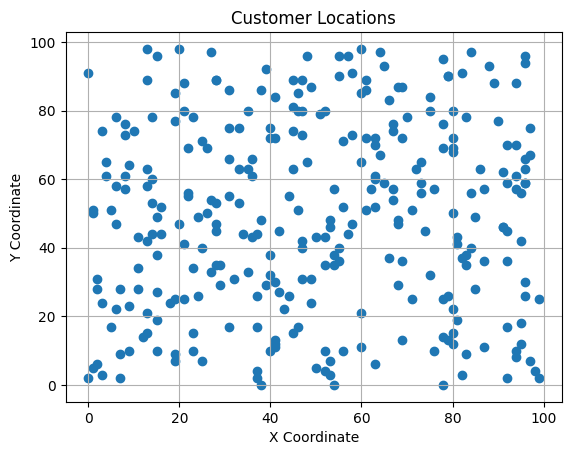
\includegraphics[width=0.45\textwidth]{WLP1.png}}
\caption{Problem uzayında dağılmış olan 300 müşterinin başlangıç lokasyonları.}
\label{fig:customers}
\end{figure}

\begin{figure}[htbp]
\centerline{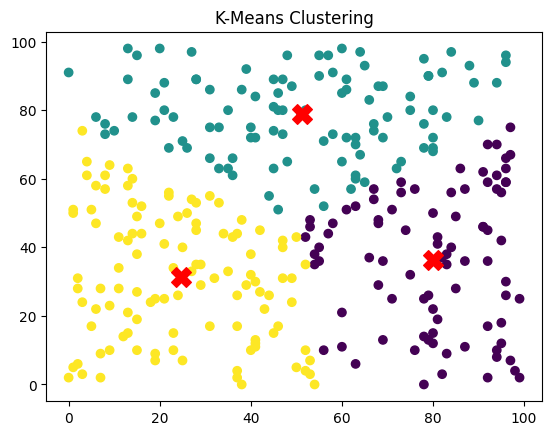
\includegraphics[width=0.45\textwidth]{WLP2.png}}
\caption{K-Means algoritması ile müşterilerin coğrafi yakınlıklarına göre kümelendirilmesi ve teorik merkez noktalarının belirlenmesi.}
\label{fig:warehouses}
\end{figure}

\begin{figure}[htbp]
\centerline{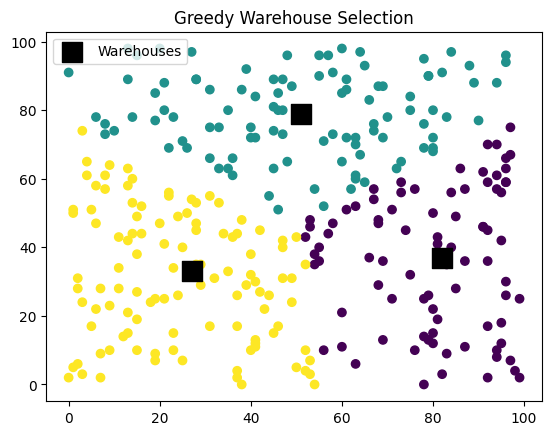
\includegraphics[width=0.45\textwidth]{WLP3.png}}
\caption{Greedy yaklaşımı sonrası belirlenen gerçek depo konumları (Siyah Kareler).}
\label{fig:warehouses}
\end{figure}

\section{Deneysel Sonuçlar ve Tartışma}

Önerilen K-Means ve Açgözlü (Greedy) entegrasyonuna dayalı hibrit lojistik modelinin başarısını doğrulamak amacıyla, arama uzayı farklı depo sayıları ($K \in \{2, 3, \dots, 8\}$) altında simüle edilmiştir. Karşılaştırma standardı (baseline) olarak kurgulanan Rastgele Arama (Random Search) algoritması, şans faktörünü minimize etmek adına her bir $K$ senaryosu için 100 bağımsız yineleme ile çalıştırılmış ve bu yinelemelerin aritmetik ortalaması ($\mu$) baz alınmıştır. Tüm deneylerde ticari gerçekçilik amacıyla depo başına sabit kurulum maliyeti $f_i = 500$ birim olarak modele dahil edilmiştir.
 
Farklı $K$ parametreleri altında algoritmaların ürettiği Mesafe Maliyeti, Sabit Maliyet ve nihai Toplam Maliyet ($TC$) çıktıları detaylı olarak Tablo I'de sunulmuştur.

\begin{table}[htbp]
\caption{Algoritmaların Maliyet ve Performans Karşılaştırması}
\begin{center}
\begin{tabular}{|c|c|c|c|}
\hline
\textbf{K} & \textbf{Mesafe} & \textbf{Sabit Tesis} & \textbf{Hibrit Toplam} \\
\textbf{Değeri} & \textbf{Maliyeti} & \textbf{Maliyeti} & \textbf{Maliyet (TC)} \\ \hline
K = 2  & 8552.42 & 1000 & 9552.42 \\ \hline
K = 3  & 6891.03 & 1500 & 8391.03 \\ \hline
K = 4  & 5681.80 & 2000 & 7681.80 \\ \hline
K = 5  & 5106.80 & 2500 & 7606.80 \\ \hline
\textbf{K = 6}  & \textbf{4565.31} & \textbf{3000} & \textbf{7565.31} \\ \hline
K = 7  & 4226.07 & 3500 & 7726.07 \\ \hline
K = 8  & 3884.82 & 4000 & 7884.82 \\ \hline
\end{tabular}
\label{tab:maliyet_tablosu}
\end{center}
\end{table}

Tablo I incelendiğinde, lojistik ağ tasarımlarındaki en temel ticaret (trade-off) mekanizması açıkça görülmektedir. Depo sayısı ($K$) arttıkça, müşteriler depolara coğrafi olarak yakınlaştığı için taşıma mesafelerinden doğan maliyetler doğrusal olarak azalmaktadır ($K=2$ için $8552.42$ birimden, $K=8$ için $3884.82$ birime düşmüştür). Ancak açılan her tesis sisteme doğrusal olarak 500 birim sabit maliyet yüklediğinden, toplam maliyet eğrisi $K=6$ noktasına kadar azalarak $7565.31$ birim ile küresel optimum (global optimum) noktasına ulaşmakta, bu noktadan sonra ise sabit tesis maliyetlerinin ($K \times 500$) baskın gelmesiyle tekrar yükselişe geçmektedir. Bu durum, sistemin 6 adet depo ile kurulmasının en ekonomik senaryo olduğunu kanıtlamaktadır.


\begin{figure}[htbp]
\centerline{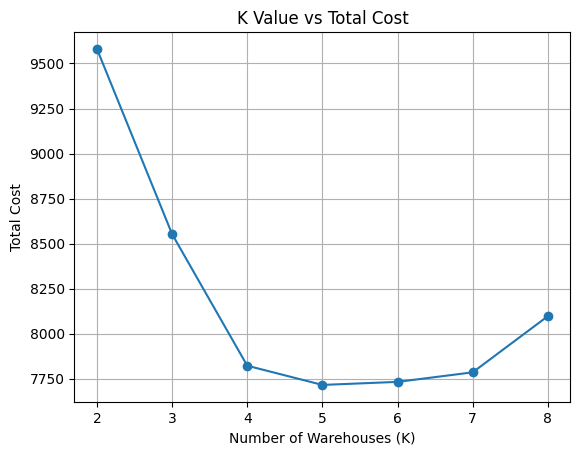
\includegraphics[width=0.45\textwidth]{WLP4.png}}
\caption{Maliyet ve depo sayısı karşılaştırılması.}
\label{fig:warehouses}
\end{figure}


Önerilen K-Means ve Açgözlü entegrasyonuna dayalı hibrit algoritmanın doğrulanması (validation) amacıyla geniş kapsamlı bir deneysel analiz mimarisi kurgulanmıştır. Algoritma kararlılığını test etmek üzere depo sayıları $K \in \{2, 3, \dots, 8\}$ aralığında parametrize edilmiştir. Hibrit modelin ürettiği çözümlerin kalitesi, her bir $K$ senaryosu için 100 bağımsız yinelemeden oluşan Monte Carlo tabanlı bir Rastgele Arama (Random Search) algoritması ile kıyaslanmıştır. Rastgele arama modelinde şans faktörünün minimize edilmesi adına 100 denemenin aritmetik ortalaması ($\mu$) baz alınmıştır. Deneyler boyunca hem taşıma (Öklid) mesafeleri hem de dinamik tesis kurulum maliyetleri ($K \times 500$) eş zamanlı olarak hesaplanarak objektif bir performans karşılaştırması elde edilmiştir.
 
Hibrit yöntem, test edilen tüm $K$ senaryolarında Rastgele Arama algoritmasının ürettiği ortalama maliyet havuzuna karşı ezici bir üstünlük sağlamış ve arama uzayını akıllıca daraltarak kurumu gereksiz maliyet yüklerinden kurtarmıştır.

% KARŞILAŞTIRMA GRAFİĞİNİN EKLENMESİ

\begin{figure}[htbp]
\centerline{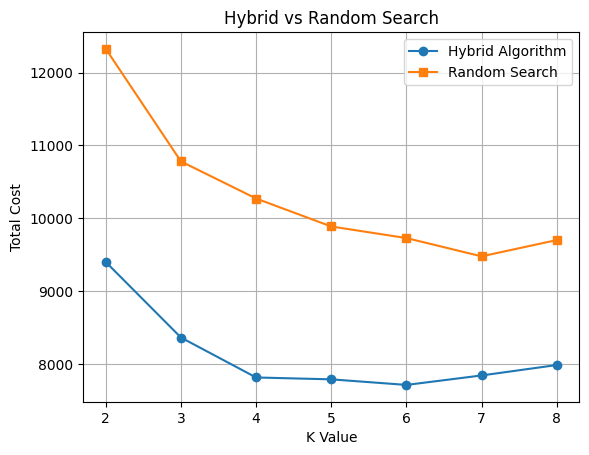
\includegraphics[width=0.48\textwidth]{WLP5.png}}
\caption{Farklı K değerlerine göre Hibrit Algoritma ve Rastgele Arama toplam maliyet değişim grafiği.}
\label{fig:comparison}
\end{figure}

\section{Sonuç ve Gelecek Çalışmalar}

Bu çalışmada, lojistik yönetiminin en kritik problemlerinden biri olan Depo Yeri Seçimi Problemi (WLP) için makine öğrenmesi ve sezgisel yaklaşımları birleştiren iki aşamalı hibrit bir optimizasyon modeli geliştirilmiştir. Sürekli uzaydaki müşteri yoğunluklarını K-Means algoritması ile anlamlı kümelere ayıran model, Açgözlü (Greedy) arama yöntemi ile bu merkezleri gerçek müşteri altyapılarına başarılı bir şekilde yerleştirmiştir.
 
Modelin ticari gerçekliğini artırmak adına sisteme dahil edilen 500 birimlik sabit tesis kurulum maliyeti kurgusu, tesis sayısı ile taşıma mesafeleri arasındaki maliyet dengesini başarıyla ortaya koymuştur. 300 müşterili sistem üzerinde gerçekleştirilen parametrik deneyler sonucunda, toplam maliyeti minimum seviyede tutan optimum depo sayısının $K=6$ olduğu saptanmıştır. Rastgele arama stratejisiyle yapılan kıyaslamalar, önerilen hibrit algoritmanın kararlı ve yüksek kaliteli çözümler ürettiğini doğrulamıştır.
 
Gelecek çalışmalarda, modele müşteri talep kapasiteleri (Capacitated Warehouse Location Problem) ve depolar arası lojistik akış kısıtları da eklenerek algoritmanın dinamik tedarik zinciri senaryolarındaki performansı incelenecektir.

\bibliographystyle{IEEEtran}
\begin{thebibliography}{00}
 
\bibitem{aboelnaga2017active}
Y. Abo-Elnaga, B. El-Sobky, and L. Al-Naser,
``An active-set trust-region algorithm for solving warehouse location problem,''
\textit{Journal of Taibah University for Science},
vol. 11, pp. 353--358, 2017.
 
\bibitem{askin2014multi}
R. G. Askin, I. Baffo, and M. Xia,
``Multi-commodity warehouse location and distribution planning with inventory consideration,''
\textit{International Journal of Production Research},
vol. 52, no. 7, pp. 1897--1910, 2014.
 
\bibitem{gill2007optimal}
A. Gill and M. I. Bhatti,
``Optimal model for warehouse location and retailer allocation,''
\textit{Applied Stochastic Models in Business and Industry},
vol. 23, pp. 213--221, 2007.
 
\bibitem{karagul2014pmedyan}
K. Karagül and R. Şahin,
``P-medyan tesis yeri seçim problemi ve çözüm yaklaşımları,'' 
ResearchGate yayını, 2014.
 
\bibitem{kalfakakou2003minimum}
R. Kalfakakou, S. Katsavounis, and K. Tsouros,
``Minimum number of warehouses for storing simultaneously compatible products,''
\textit{International Journal of Production Economics},
vol. 81--82, pp. 559--564, 2003.
 
\bibitem{kmeans}
``K-Ortalamalar yönteminin başlangıç merkez seçim sorunsalı üzerine bir çalışma,''
ResearchGate yayını, erişim tarihi: 20 Mayıs 2026.
 
\bibitem{michel2004simple}
L. Michel and P. Van Hentenryck,
``A simple tabu search for warehouse location,''
\textit{European Journal of Operational Research},
vol. 157, pp. 576--591, 2004.
 
\bibitem{owen1998strategic}
S. H. Owen and M. S. Daskin,
``Strategic facility location: A review,''
\textit{European Journal of Operational Research},
vol. 111, no. 3, pp. 423--447, 1998.
 
\bibitem{rath2014math}
S. Rath and W. J. Gutjahr,
``A math-heuristic for the warehouse location-routing problem in disaster relief,''
\textit{Computers \& Operations Research},
vol. 42, pp. 25--39, 2014.
 
\bibitem{sagnak2020depo}
M. Sağnak,
``Depo yeri seçimi: Perakende sektöründe melez çok kriterli karar verme uygulaması,''
\textit{Yaşar Üniversitesi E-Dergisi},
vol. 15, no. 59, pp. 615--623, 2020.
 
\bibitem{salhi2003genetic}
S. Salhi and M. D. H. Gamal,
``A genetic algorithm based approach for the uncapacitated continuous location-allocation problem,''
\textit{Annals of Operations Research},
vol. 123, no. 1, pp. 203--222, 2003.
 
\bibitem{yaobao2013improved}
Z. Yaobao, H. Ping, and Y. Shu,
``An improved particle swarm optimization for the automobile spare part warehouse location problem,''
\textit{Mathematical Problems in Engineering},
vol. 2013, Article 726194, 2013.
 
\bibitem{you2019optimal}
M. You, Y. Xiao, S. Zhang, P. Yang, and S. Zhou,
``Optimal mathematical programming for the warehouse location problem with Euclidean distance linearization,''
\textit{Computers \& Industrial Engineering},
vol. 136, pp. 70--79, 2019.
 
\end{thebibliography}

\end{document}

\end{document}

\author{\IEEEauthorblockN{1\textsuperscript{st} Given Name Surname}
\IEEEauthorblockA{\textit{dept. name of organization (of Aff.)} \\
\textit{name of organization (of Aff.)}\\
City, Country \\
email address or ORCID}
\and
\IEEEauthorblockN{2\textsuperscript{nd} Given Name Surname}
\IEEEauthorblockA{\textit{dept. name of organization (of Aff.)} \\
\textit{name of organization (of Aff.)}\\
City, Country \\
email address or ORCID}
\and
\IEEEauthorblockN{3\textsuperscript{rd} Given Name Surname}
\IEEEauthorblockA{\textit{dept. name of organization (of Aff.)} \\
\textit{name of organization (of Aff.)}\\
City, Country \\
email address or ORCID}
\and
\IEEEauthorblockN{4\textsuperscript{th} Given Name Surname}
\IEEEauthorblockA{\textit{dept. name of organization (of Aff.)} \\
\textit{name of organization (of Aff.)}\\
City, Country \\
email address or ORCID}
\and
\IEEEauthorblockN{5\textsuperscript{th} Given Name Surname}
\IEEEauthorblockA{\textit{dept. name of organization (of Aff.)} \\
\textit{name of organization (of Aff.)}\\
City, Country \\
email address or ORCID}
\and
\IEEEauthorblockN{6\textsuperscript{th} Given Name Surname}
\IEEEauthorblockA{\textit{dept. name of organization (of Aff.)} \\
\textit{name of organization (of Aff.)}\\
City, Country \\
email address or ORCID}
}

\maketitle

\begin{abstract}
This document is a model and instructions for \LaTeX.
This and the IEEEtran.cls file define the components of your paper [title, text, heads, etc.]. *CRITICAL: Do Not Use Symbols, Special Characters, Footnotes, 
or Math in Paper Title or Abstract.
\end{abstract}

\begin{IEEEkeywords}
component, formatting, style, styling, insert
\end{IEEEkeywords}

\section{Introduction}
This document is a model and instructions for \LaTeX.
Please observe the conference page limits. 

\section{Ease of Use}

\subsection{Maintaining the Integrity of the Specifications}

The IEEEtran class file is used to format your paper and style the text. All margins, 
column widths, line spaces, and text fonts are prescribed; please do not 
alter them. You may note peculiarities. For example, the head margin
measures proportionately more than is customary. This measurement 
and others are deliberate, using specifications that anticipate your paper 
as one part of the entire proceedings, and not as an independent document. 
Please do not revise any of the current designations.

\section{Prepare Your Paper Before Styling}
Before you begin to format your paper, first write and save the content as a 
separate text file. Complete all content and organizational editing before 
formatting. Please note sections \ref{AA}--\ref{SCM} below for more information on 
proofreading, spelling and grammar.

Keep your text and graphic files separate until after the text has been 
formatted and styled. Do not number text heads---{\LaTeX} will do that 
for you.

\subsection{Abbreviations and Acronyms}\label{AA}
Define abbreviations and acronyms the first time they are used in the text, 
even after they have been defined in the abstract. Abbreviations such as 
IEEE, SI, MKS, CGS, ac, dc, and rms do not have to be defined. Do not use 
abbreviations in the title or heads unless they are unavoidable.

\subsection{Units}
\begin{itemize}
\item Use either SI (MKS) or CGS as primary units. (SI units are encouraged.) English units may be used as secondary units (in parentheses). An exception would be the use of English units as identifiers in trade, such as ``3.5-inch disk drive''.
\item Avoid combining SI and CGS units, such as current in amperes and magnetic field in oersteds. This often leads to confusion because equations do not balance dimensionally. If you must use mixed units, clearly state the units for each quantity that you use in an equation.
\item Do not mix complete spellings and abbreviations of units: ``Wb/m\textsuperscript{2}'' or ``webers per square meter'', not ``webers/m\textsuperscript{2}''. Spell out units when they appear in text: ``. . . a few henries'', not ``. . . a few H''.
\item Use a zero before decimal points: ``0.25'', not ``.25''. Use ``cm\textsuperscript{3}'', not ``cc''.)
\end{itemize}

\subsection{Equations}
Number equations consecutively. To make your 
equations more compact, you may use the solidus (~/~), the exp function, or 
appropriate exponents. Italicize Roman symbols for quantities and variables, 
but not Greek symbols. Use a long dash rather than a hyphen for a minus 
sign. Punctuate equations with commas or periods when they are part of a 
sentence, as in:
\begin{equation}
a+b=\gamma\label{eq}
\end{equation}

Be sure that the 
symbols in your equation have been defined before or immediately following 
the equation. Use ``\eqref{eq}'', not ``Eq.~\eqref{eq}'' or ``equation \eqref{eq}'', except at 
the beginning of a sentence: ``Equation \eqref{eq} is . . .''

\subsection{\LaTeX-Specific Advice}

Please use ``soft'' (e.g., \verb|\eqref{Eq}|) cross references instead
of ``hard'' references (e.g., \verb|(1)|). That will make it possible
to combine sections, add equations, or change the order of figures or
citations without having to go through the file line by line.

Please don't use the \verb|{eqnarray}| equation environment. Use
\verb|{align}| or \verb|{IEEEeqnarray}| instead. The \verb|{eqnarray}|
environment leaves unsightly spaces around relation symbols.

Please note that the \verb|{subequations}| environment in {\LaTeX}
will increment the main equation counter even when there are no
equation numbers displayed. If you forget that, you might write an
article in which the equation numbers skip from (17) to (20), causing
the copy editors to wonder if you've discovered a new method of
counting.

{\BibTeX} does not work by magic. It doesn't get the bibliographic
data from thin air but from .bib files. If you use {\BibTeX} to produce a
bibliography you must send the .bib files. 

{\LaTeX} can't read your mind. If you assign the same label to a
subsubsection and a table, you might find that Table I has been cross
referenced as Table IV-B3. 

{\LaTeX} does not have precognitive abilities. If you put a
\verb|\label| command before the command that updates the counter it's
supposed to be using, the label will pick up the last counter to be
cross referenced instead. In particular, a \verb|\label| command
should not go before the caption of a figure or a table.

Do not use \verb|\nonumber| inside the \verb|{array}| environment. It
will not stop equation numbers inside \verb|{array}| (there won't be
any anyway) and it might stop a wanted equation number in the
surrounding equation.

\subsection{Some Common Mistakes}\label{SCM}
\begin{itemize}
\item The word ``data'' is plural, not singular.
\item The subscript for the permeability of vacuum $\mu_{0}$, and other common scientific constants, is zero with subscript formatting, not a lowercase letter ``o''.
\item In American English, commas, semicolons, periods, question and exclamation marks are located within quotation marks only when a complete thought or name is cited, such as a title or full quotation. When quotation marks are used, instead of a bold or italic typeface, to highlight a word or phrase, punctuation should appear outside of the quotation marks. A parenthetical phrase or statement at the end of a sentence is punctuated outside of the closing parenthesis (like this). (A parenthetical sentence is punctuated within the parentheses.)
\item A graph within a graph is an ``inset'', not an ``insert''. The word alternatively is preferred to the word ``alternately'' (unless you really mean something that alternates).
\item Do not use the word ``essentially'' to mean ``approximately'' or ``effectively''.
\item In your paper title, if the words ``that uses'' can accurately replace the word ``using'', capitalize the ``u''; if not, keep using lower-cased.
\item Be aware of the different meanings of the homophones ``affect'' and ``effect'', ``complement'' and ``compliment'', ``discreet'' and ``discrete'', ``principal'' and ``principle''.
\item Do not confuse ``imply'' and ``infer''.
\item The prefix ``non'' is not a word; it should be joined to the word it modifies, usually without a hyphen.
\item There is no period after the ``et'' in the Latin abbreviation ``et al.''.
\item The abbreviation ``i.e.'' means ``that is'', and the abbreviation ``e.g.'' means ``for example''.
\end{itemize}
An excellent style manual for science writers is \cite{b7}.

\subsection{Authors and Affiliations}
\textbf{The class file is designed for, but not limited to, six authors.} A 
minimum of one author is required for all conference articles. Author names 
should be listed starting from left to right and then moving down to the 
next line. This is the author sequence that will be used in future citations 
and by indexing services. Names should not be listed in columns nor group by 
affiliation. Please keep your affiliations as succinct as possible (for 
example, do not differentiate among departments of the same organization).

\subsection{Identify the Headings}
Headings, or heads, are organizational devices that guide the reader through 
your paper. There are two types: component heads and text heads.

Component heads identify the different components of your paper and are not 
topically subordinate to each other. Examples include Acknowledgments and 
References and, for these, the correct style to use is ``Heading 5''. Use 
``figure caption'' for your Figure captions, and ``table head'' for your 
table title. Run-in heads, such as ``Abstract'', will require you to apply a 
style (in this case, italic) in addition to the style provided by the drop 
down menu to differentiate the head from the text.

Text heads organize the topics on a relational, hierarchical basis. For 
example, the paper title is the primary text head because all subsequent 
material relates and elaborates on this one topic. If there are two or more 
sub-topics, the next level head (uppercase Roman numerals) should be used 
and, conversely, if there are not at least two sub-topics, then no subheads 
should be introduced.

\subsection{Figures and Tables}
\paragraph{Positioning Figures and Tables} Place figures and tables at the top and 
bottom of columns. Avoid placing them in the middle of columns. Large 
figures and tables may span across both columns. Figure captions should be 
below the figures; table heads should appear above the tables. Insert 
figures and tables after they are cited in the text. Use the abbreviation 
``Fig.~\ref{fig}'', even at the beginning of a sentence.

\begin{table}[htbp]
\caption{Table Type Styles}
\begin{center}
\begin{tabular}{|c|c|c|c|}
\hline
\textbf{Table}&\multicolumn{3}{|c|}{\textbf{Table Column Head}} \\
\cline{2-4} 
\textbf{Head} & \textbf{\textit{Table column subhead}}& \textbf{\textit{Subhead}}& \textbf{\textit{Subhead}} \\
\hline
copy& More table copy$^{\mathrm{a}}$& &  \\
\hline
\multicolumn{4}{l}{$^{\mathrm{a}}$Sample of a Table footnote.}
\end{tabular}
\label{tab1}
\end{center}
\end{table}

\begin{figure}[htbp]
\centerline{
\includegraphics{fig1.png}}
\caption{Example of a figure caption.}
\label{fig}
\end{figure}

Figure Labels: Use 8 point Times New Roman for Figure labels. Use words 
rather than symbols or abbreviations when writing Figure axis labels to 
avoid confusing the reader. As an example, write the quantity 
``Magnetization'', or ``Magnetization, M'', not just ``M''. If including 
units in the label, present them within parentheses. Do not label axes only 
with units. In the example, write ``Magnetization (A/m)'' or ``Magnetization 
\{A[m(1)]\}'', not just ``A/m''. Do not label axes with a ratio of 
quantities and units. For example, write ``Temperature (K)'', not 
``Temperature/K''.

\section*{Acknowledgment}

The preferred spelling of the word ``acknowledgment'' in America is without 
an ``e'' after the ``g''. Avoid the stilted expression ``one of us (R. B. 
G.) thanks $\ldots$''. Instead, try ``R. B. G. thanks$\ldots$''. Put sponsor 
acknowledgments in the unnumbered footnote on the first page.

\section*{References}

Please number citations consecutively within brackets \cite{b1}. The 
sentence punctuation follows the bracket \cite{b2}. Refer simply to the reference 
number, as in \cite{b3}---do not use ``Ref. \cite{b3}'' or ``reference \cite{b3}'' except at 
the beginning of a sentence: ``Reference \cite{b3} was the first $\ldots$''

Number footnotes separately in superscripts. Place the actual footnote at 
the bottom of the column in which it was cited. Do not put footnotes in the 
abstract or reference list. Use letters for table footnotes.

Unless there are six authors or more give all authors' names; do not use 
``et al.''. Papers that have not been published, even if they have been 
submitted for publication, should be cited as ``unpublished'' \cite{b4}. Papers 
that have been accepted for publication should be cited as ``in press'' \cite{b5}. 
Capitalize only the first word in a paper title, except for proper nouns and 
element symbols.

For papers published in translation journals, please give the English 
citation first, followed by the original foreign-language citation \cite{b6}.

\begin{thebibliography}{00}
\bibitem{b1} G. Eason, B. Noble, and I. N. Sneddon, ``On certain integrals of Lipschitz-Hankel type involving products of Bessel functions,'' Phil. Trans. Roy. Soc. London, vol. A247, pp. 529--551, April 1955.
\bibitem{b2} J. Clerk Maxwell, A Treatise on Electricity and Magnetism, 3rd ed., vol. 2. Oxford: Clarendon, 1892, pp.68--73.
\bibitem{b3} I. S. Jacobs and C. P. Bean, ``Fine particles, thin films and exchange anisotropy,'' in Magnetism, vol. III, G. T. Rado and H. Suhl, Eds. New York: Academic, 1963, pp. 271--350.
\bibitem{b4} K. Elissa, ``Title of paper if known,'' unpublished.
\bibitem{b5} R. Nicole, ``Title of paper with only first word capitalized,'' J. Name Stand. Abbrev., in press.
\bibitem{b6} Y. Yorozu, M. Hirano, K. Oka, and Y. Tagawa, ``Electron spectroscopy studies on magneto-optical media and plastic substrate interface,'' IEEE Transl. J. Magn. Japan, vol. 2, pp. 740--741, August 1987 [Digests 9th Annual Conf. Magnetics Japan, p. 301, 1982].
\bibitem{b7} M. Young, The Technical Writer's Handbook. Mill Valley, CA: University Science, 1989.
\end{thebibliography}
\vspace{12pt}
\color{red}
IEEE conference templates contain guidance text for composing and formatting conference papers. Please ensure that all template text is removed from your conference paper prior to submission to the conference. Failure to remove the template text from your paper may result in your paper not being published.

\end{document}
